\DeclareUnicodeCharacter{041B}{\CYRL}



\documentclass[11pt]{article}

    
    
    \usepackage[breakable]{tcolorbox}
    \usepackage{parskip} % Stop auto-indenting (to mimic markdown behaviour)
    \usepackage[english,russian]{babel}
    \usepackage{graphicx}
    \usepackage{subcaption}
    

    % Basic figure setup, for now with no caption control since it's done
    % automatically by Pandoc (which extracts ![](path) syntax from Markdown).
    \usepackage{graphicx}
    % Maintain compatibility with old templates. Remove in nbconvert 6.0
    \let\Oldincludegraphics\includegraphics
    % Ensure that by default, figures have no caption (until we provide a
    % proper Figure object with a Caption API and a way to capture that
    % in the conversion process - todo).
    \usepackage{caption}
    \DeclareCaptionFormat{nocaption}{}
    \captionsetup{format=nocaption,aboveskip=0pt,belowskip=0pt}

    \usepackage{float}
    \floatplacement{figure}{H} % forces figures to be placed at the correct location
    \usepackage{xcolor} % Allow colors to be defined
    \usepackage{enumerate} % Needed for markdown enumerations to work
    \usepackage{geometry} % Used to adjust the document margins
    \usepackage{amsmath} % Equations
    \usepackage{amssymb} % Equations
    \usepackage{textcomp} % defines textquotesingle
    % Hack from http://tex.stackexchange.com/a/47451/13684:
    \AtBeginDocument{%
        \def\PYZsq{\textquotesingle}% Upright quotes in Pygmentized code
    }
    \usepackage{upquote} % Upright quotes for verbatim code
    \usepackage{eurosym} % defines \euro

    \usepackage{iftex}
    \ifPDFTeX
        \usepackage[T1]{fontenc}
        \IfFileExists{alphabeta.sty}{
              \usepackage{alphabeta}
          }{
              \usepackage[mathletters]{ucs}
              \usepackage[utf8x]{inputenc}
          }
    \else
        \usepackage{fontspec}
        \usepackage{unicode-math}
    \fi

    \usepackage{fancyvrb} % verbatim replacement that allows latex
    \usepackage{grffile} % extends the file name processing of package graphics
                         % to support a larger range
    \makeatletter % fix for old versions of grffile with XeLaTeX
    \@ifpackagelater{grffile}{2019/11/01}
    {
      % Do nothing on new versions
    }
    {
      \def\Gread@@xetex#1{%
        \IfFileExists{"\Gin@base".bb}%
        {\Gread@eps{\Gin@base.bb}}%
        {\Gread@@xetex@aux#1}%
      }
    }
    \makeatother
    \usepackage[Export]{adjustbox} % Used to constrain images to a maximum size
    \adjustboxset{max size={0.9\linewidth}{0.9\paperheight}}

    % The hyperref package gives us a pdf with properly built
    % internal navigation ('pdf bookmarks' for the table of contents,
    % internal cross-reference links, web links for URLs, etc.)
    \usepackage{hyperref}
    % The default LaTeX title has an obnoxious amount of whitespace. By default,
    % titling removes some of it. It also provides customization options.
    \usepackage{titling}
    \usepackage{longtable} % longtable support required by pandoc >1.10
    \usepackage{booktabs}  % table support for pandoc > 1.12.2
    \usepackage{array}     % table support for pandoc >= 2.11.3
    \usepackage{calc}      % table minipage width calculation for pandoc >= 2.11.1
    \usepackage[inline]{enumitem} % IRkernel/repr support (it uses the enumerate* environment)
    \usepackage[normalem]{ulem} % ulem is needed to support strikethroughs (\sout)
                                % normalem makes italics be italics, not underlines
    \usepackage{mathrsfs}
    

    
    % Colors for the hyperref package
    \definecolor{urlcolor}{rgb}{0,.145,.698}
    \definecolor{linkcolor}{rgb}{.71,0.21,0.01}
    \definecolor{citecolor}{rgb}{.12,.54,.11}

    % ANSI colors
    \definecolor{ansi-black}{HTML}{3E424D}
    \definecolor{ansi-black-intense}{HTML}{282C36}
    \definecolor{ansi-red}{HTML}{E75C58}
    \definecolor{ansi-red-intense}{HTML}{B22B31}
    \definecolor{ansi-green}{HTML}{00A250}
    \definecolor{ansi-green-intense}{HTML}{007427}
    \definecolor{ansi-yellow}{HTML}{DDB62B}
    \definecolor{ansi-yellow-intense}{HTML}{B27D12}
    \definecolor{ansi-blue}{HTML}{208FFB}
    \definecolor{ansi-blue-intense}{HTML}{0065CA}
    \definecolor{ansi-magenta}{HTML}{D160C4}
    \definecolor{ansi-magenta-intense}{HTML}{A03196}
    \definecolor{ansi-cyan}{HTML}{60C6C8}
    \definecolor{ansi-cyan-intense}{HTML}{258F8F}
    \definecolor{ansi-white}{HTML}{C5C1B4}
    \definecolor{ansi-white-intense}{HTML}{A1A6B2}
    \definecolor{ansi-default-inverse-fg}{HTML}{FFFFFF}
    \definecolor{ansi-default-inverse-bg}{HTML}{000000}

    % common color for the border for error outputs.
    \definecolor{outerrorbackground}{HTML}{FFDFDF}

    % commands and environments needed by pandoc snippets
    % extracted from the output of `pandoc -s`
    \providecommand{\tightlist}{%
      \setlength{\itemsep}{0pt}\setlength{\parskip}{0pt}}
    \DefineVerbatimEnvironment{Highlighting}{Verbatim}{commandchars=\\\{\}}
    % Add ',fontsize=\small' for more characters per line
    \newenvironment{Shaded}{}{}
    \newcommand{\KeywordTok}[1]{\textcolor[rgb]{0.00,0.44,0.13}{\textbf{{#1}}}}
    \newcommand{\DataTypeTok}[1]{\textcolor[rgb]{0.56,0.13,0.00}{{#1}}}
    \newcommand{\DecValTok}[1]{\textcolor[rgb]{0.25,0.63,0.44}{{#1}}}
    \newcommand{\BaseNTok}[1]{\textcolor[rgb]{0.25,0.63,0.44}{{#1}}}
    \newcommand{\FloatTok}[1]{\textcolor[rgb]{0.25,0.63,0.44}{{#1}}}
    \newcommand{\CharTok}[1]{\textcolor[rgb]{0.25,0.44,0.63}{{#1}}}
    \newcommand{\StringTok}[1]{\textcolor[rgb]{0.25,0.44,0.63}{{#1}}}
    \newcommand{\CommentTok}[1]{\textcolor[rgb]{0.38,0.63,0.69}{\textit{{#1}}}}
    \newcommand{\OtherTok}[1]{\textcolor[rgb]{0.00,0.44,0.13}{{#1}}}
    \newcommand{\AlertTok}[1]{\textcolor[rgb]{1.00,0.00,0.00}{\textbf{{#1}}}}
    \newcommand{\FunctionTok}[1]{\textcolor[rgb]{0.02,0.16,0.49}{{#1}}}
    \newcommand{\RegionMarkerTok}[1]{{#1}}
    \newcommand{\ErrorTok}[1]{\textcolor[rgb]{1.00,0.00,0.00}{\textbf{{#1}}}}
    \newcommand{\NormalTok}[1]{{#1}}

    % Additional commands for more recent versions of Pandoc
    \newcommand{\ConstantTok}[1]{\textcolor[rgb]{0.53,0.00,0.00}{{#1}}}
    \newcommand{\SpecialCharTok}[1]{\textcolor[rgb]{0.25,0.44,0.63}{{#1}}}
    \newcommand{\VerbatimStringTok}[1]{\textcolor[rgb]{0.25,0.44,0.63}{{#1}}}
    \newcommand{\SpecialStringTok}[1]{\textcolor[rgb]{0.73,0.40,0.53}{{#1}}}
    \newcommand{\ImportTok}[1]{{#1}}
    \newcommand{\DocumentationTok}[1]{\textcolor[rgb]{0.73,0.13,0.13}{\textit{{#1}}}}
    \newcommand{\AnnotationTok}[1]{\textcolor[rgb]{0.38,0.63,0.69}{\textbf{\textit{{#1}}}}}
    \newcommand{\CommentVarTok}[1]{\textcolor[rgb]{0.38,0.63,0.69}{\textbf{\textit{{#1}}}}}
    \newcommand{\VariableTok}[1]{\textcolor[rgb]{0.10,0.09,0.49}{{#1}}}
    \newcommand{\ControlFlowTok}[1]{\textcolor[rgb]{0.00,0.44,0.13}{\textbf{{#1}}}}
    \newcommand{\OperatorTok}[1]{\textcolor[rgb]{0.40,0.40,0.40}{{#1}}}
    \newcommand{\BuiltInTok}[1]{{#1}}
    \newcommand{\ExtensionTok}[1]{{#1}}
    \newcommand{\PreprocessorTok}[1]{\textcolor[rgb]{0.74,0.48,0.00}{{#1}}}
    \newcommand{\AttributeTok}[1]{\textcolor[rgb]{0.49,0.56,0.16}{{#1}}}
    \newcommand{\InformationTok}[1]{\textcolor[rgb]{0.38,0.63,0.69}{\textbf{\textit{{#1}}}}}
    \newcommand{\WarningTok}[1]{\textcolor[rgb]{0.38,0.63,0.69}{\textbf{\textit{{#1}}}}}


    % Define a nice break command that doesn't care if a line doesn't already
    % exist.
    \def\br{\hspace*{\fill} \\* }
    % Math Jax compatibility definitions
    \def\gt{>}
    \def\lt{<}
    \let\Oldtex\TeX
    \let\Oldlatex\LaTeX
    \renewcommand{\TeX}{\textrm{\Oldtex}}
    \renewcommand{\LaTeX}{\textrm{\Oldlatex}}
    % Document parameters
    % Document title
    \title{CHM\_Lab1}
    
    
    
    
    
% Pygments definitions
\makeatletter
\def\PY@reset{\let\PY@it=\relax \let\PY@bf=\relax%
    \let\PY@ul=\relax \let\PY@tc=\relax%
    \let\PY@bc=\relax \let\PY@ff=\relax}
\def\PY@tok#1{\csname PY@tok@#1\endcsname}
\def\PY@toks#1+{\ifx\relax#1\empty\else%
    \PY@tok{#1}\expandafter\PY@toks\fi}
\def\PY@do#1{\PY@bc{\PY@tc{\PY@ul{%
    \PY@it{\PY@bf{\PY@ff{#1}}}}}}}
\def\PY#1#2{\PY@reset\PY@toks#1+\relax+\PY@do{#2}}

\@namedef{PY@tok@w}{\def\PY@tc##1{\textcolor[rgb]{0.73,0.73,0.73}{##1}}}
\@namedef{PY@tok@c}{\let\PY@it=\textit\def\PY@tc##1{\textcolor[rgb]{0.24,0.48,0.48}{##1}}}
\@namedef{PY@tok@cp}{\def\PY@tc##1{\textcolor[rgb]{0.61,0.40,0.00}{##1}}}
\@namedef{PY@tok@k}{\let\PY@bf=\textbf\def\PY@tc##1{\textcolor[rgb]{0.00,0.50,0.00}{##1}}}
\@namedef{PY@tok@kp}{\def\PY@tc##1{\textcolor[rgb]{0.00,0.50,0.00}{##1}}}
\@namedef{PY@tok@kt}{\def\PY@tc##1{\textcolor[rgb]{0.69,0.00,0.25}{##1}}}
\@namedef{PY@tok@o}{\def\PY@tc##1{\textcolor[rgb]{0.40,0.40,0.40}{##1}}}
\@namedef{PY@tok@ow}{\let\PY@bf=\textbf\def\PY@tc##1{\textcolor[rgb]{0.67,0.13,1.00}{##1}}}
\@namedef{PY@tok@nb}{\def\PY@tc##1{\textcolor[rgb]{0.00,0.50,0.00}{##1}}}
\@namedef{PY@tok@nf}{\def\PY@tc##1{\textcolor[rgb]{0.00,0.00,1.00}{##1}}}
\@namedef{PY@tok@nc}{\let\PY@bf=\textbf\def\PY@tc##1{\textcolor[rgb]{0.00,0.00,1.00}{##1}}}
\@namedef{PY@tok@nn}{\let\PY@bf=\textbf\def\PY@tc##1{\textcolor[rgb]{0.00,0.00,1.00}{##1}}}
\@namedef{PY@tok@ne}{\let\PY@bf=\textbf\def\PY@tc##1{\textcolor[rgb]{0.80,0.25,0.22}{##1}}}
\@namedef{PY@tok@nv}{\def\PY@tc##1{\textcolor[rgb]{0.10,0.09,0.49}{##1}}}
\@namedef{PY@tok@no}{\def\PY@tc##1{\textcolor[rgb]{0.53,0.00,0.00}{##1}}}
\@namedef{PY@tok@nl}{\def\PY@tc##1{\textcolor[rgb]{0.46,0.46,0.00}{##1}}}
\@namedef{PY@tok@ni}{\let\PY@bf=\textbf\def\PY@tc##1{\textcolor[rgb]{0.44,0.44,0.44}{##1}}}
\@namedef{PY@tok@na}{\def\PY@tc##1{\textcolor[rgb]{0.41,0.47,0.13}{##1}}}
\@namedef{PY@tok@nt}{\let\PY@bf=\textbf\def\PY@tc##1{\textcolor[rgb]{0.00,0.50,0.00}{##1}}}
\@namedef{PY@tok@nd}{\def\PY@tc##1{\textcolor[rgb]{0.67,0.13,1.00}{##1}}}
\@namedef{PY@tok@s}{\def\PY@tc##1{\textcolor[rgb]{0.73,0.13,0.13}{##1}}}
\@namedef{PY@tok@sd}{\let\PY@it=\textit\def\PY@tc##1{\textcolor[rgb]{0.73,0.13,0.13}{##1}}}
\@namedef{PY@tok@si}{\let\PY@bf=\textbf\def\PY@tc##1{\textcolor[rgb]{0.64,0.35,0.47}{##1}}}
\@namedef{PY@tok@se}{\let\PY@bf=\textbf\def\PY@tc##1{\textcolor[rgb]{0.67,0.36,0.12}{##1}}}
\@namedef{PY@tok@sr}{\def\PY@tc##1{\textcolor[rgb]{0.64,0.35,0.47}{##1}}}
\@namedef{PY@tok@ss}{\def\PY@tc##1{\textcolor[rgb]{0.10,0.09,0.49}{##1}}}
\@namedef{PY@tok@sx}{\def\PY@tc##1{\textcolor[rgb]{0.00,0.50,0.00}{##1}}}
\@namedef{PY@tok@m}{\def\PY@tc##1{\textcolor[rgb]{0.40,0.40,0.40}{##1}}}
\@namedef{PY@tok@gh}{\let\PY@bf=\textbf\def\PY@tc##1{\textcolor[rgb]{0.00,0.00,0.50}{##1}}}
\@namedef{PY@tok@gu}{\let\PY@bf=\textbf\def\PY@tc##1{\textcolor[rgb]{0.50,0.00,0.50}{##1}}}
\@namedef{PY@tok@gd}{\def\PY@tc##1{\textcolor[rgb]{0.63,0.00,0.00}{##1}}}
\@namedef{PY@tok@gi}{\def\PY@tc##1{\textcolor[rgb]{0.00,0.52,0.00}{##1}}}
\@namedef{PY@tok@gr}{\def\PY@tc##1{\textcolor[rgb]{0.89,0.00,0.00}{##1}}}
\@namedef{PY@tok@ge}{\let\PY@it=\textit}
\@namedef{PY@tok@gs}{\let\PY@bf=\textbf}
\@namedef{PY@tok@gp}{\let\PY@bf=\textbf\def\PY@tc##1{\textcolor[rgb]{0.00,0.00,0.50}{##1}}}
\@namedef{PY@tok@go}{\def\PY@tc##1{\textcolor[rgb]{0.44,0.44,0.44}{##1}}}
\@namedef{PY@tok@gt}{\def\PY@tc##1{\textcolor[rgb]{0.00,0.27,0.87}{##1}}}
\@namedef{PY@tok@err}{\def\PY@bc##1{{\setlength{\fboxsep}{\string -\fboxrule}\fcolorbox[rgb]{1.00,0.00,0.00}{1,1,1}{\strut ##1}}}}
\@namedef{PY@tok@kc}{\let\PY@bf=\textbf\def\PY@tc##1{\textcolor[rgb]{0.00,0.50,0.00}{##1}}}
\@namedef{PY@tok@kd}{\let\PY@bf=\textbf\def\PY@tc##1{\textcolor[rgb]{0.00,0.50,0.00}{##1}}}
\@namedef{PY@tok@kn}{\let\PY@bf=\textbf\def\PY@tc##1{\textcolor[rgb]{0.00,0.50,0.00}{##1}}}
\@namedef{PY@tok@kr}{\let\PY@bf=\textbf\def\PY@tc##1{\textcolor[rgb]{0.00,0.50,0.00}{##1}}}
\@namedef{PY@tok@bp}{\def\PY@tc##1{\textcolor[rgb]{0.00,0.50,0.00}{##1}}}
\@namedef{PY@tok@fm}{\def\PY@tc##1{\textcolor[rgb]{0.00,0.00,1.00}{##1}}}
\@namedef{PY@tok@vc}{\def\PY@tc##1{\textcolor[rgb]{0.10,0.09,0.49}{##1}}}
\@namedef{PY@tok@vg}{\def\PY@tc##1{\textcolor[rgb]{0.10,0.09,0.49}{##1}}}
\@namedef{PY@tok@vi}{\def\PY@tc##1{\textcolor[rgb]{0.10,0.09,0.49}{##1}}}
\@namedef{PY@tok@vm}{\def\PY@tc##1{\textcolor[rgb]{0.10,0.09,0.49}{##1}}}
\@namedef{PY@tok@sa}{\def\PY@tc##1{\textcolor[rgb]{0.73,0.13,0.13}{##1}}}
\@namedef{PY@tok@sb}{\def\PY@tc##1{\textcolor[rgb]{0.73,0.13,0.13}{##1}}}
\@namedef{PY@tok@sc}{\def\PY@tc##1{\textcolor[rgb]{0.73,0.13,0.13}{##1}}}
\@namedef{PY@tok@dl}{\def\PY@tc##1{\textcolor[rgb]{0.73,0.13,0.13}{##1}}}
\@namedef{PY@tok@s2}{\def\PY@tc##1{\textcolor[rgb]{0.73,0.13,0.13}{##1}}}
\@namedef{PY@tok@sh}{\def\PY@tc##1{\textcolor[rgb]{0.73,0.13,0.13}{##1}}}
\@namedef{PY@tok@s1}{\def\PY@tc##1{\textcolor[rgb]{0.73,0.13,0.13}{##1}}}
\@namedef{PY@tok@mb}{\def\PY@tc##1{\textcolor[rgb]{0.40,0.40,0.40}{##1}}}
\@namedef{PY@tok@mf}{\def\PY@tc##1{\textcolor[rgb]{0.40,0.40,0.40}{##1}}}
\@namedef{PY@tok@mh}{\def\PY@tc##1{\textcolor[rgb]{0.40,0.40,0.40}{##1}}}
\@namedef{PY@tok@mi}{\def\PY@tc##1{\textcolor[rgb]{0.40,0.40,0.40}{##1}}}
\@namedef{PY@tok@il}{\def\PY@tc##1{\textcolor[rgb]{0.40,0.40,0.40}{##1}}}
\@namedef{PY@tok@mo}{\def\PY@tc##1{\textcolor[rgb]{0.40,0.40,0.40}{##1}}}
\@namedef{PY@tok@ch}{\let\PY@it=\textit\def\PY@tc##1{\textcolor[rgb]{0.24,0.48,0.48}{##1}}}
\@namedef{PY@tok@cm}{\let\PY@it=\textit\def\PY@tc##1{\textcolor[rgb]{0.24,0.48,0.48}{##1}}}
\@namedef{PY@tok@cpf}{\let\PY@it=\textit\def\PY@tc##1{\textcolor[rgb]{0.24,0.48,0.48}{##1}}}
\@namedef{PY@tok@c1}{\let\PY@it=\textit\def\PY@tc##1{\textcolor[rgb]{0.24,0.48,0.48}{##1}}}
\@namedef{PY@tok@cs}{\let\PY@it=\textit\def\PY@tc##1{\textcolor[rgb]{0.24,0.48,0.48}{##1}}}

\def\PYZbs{\char`\\}
\def\PYZus{\char`\_}
\def\PYZob{\char`\{}
\def\PYZcb{\char`\}}
\def\PYZca{\char`\^}
\def\PYZam{\char`\&}
\def\PYZlt{\char`\<}
\def\PYZgt{\char`\>}
\def\PYZsh{\char`\#}
\def\PYZpc{\char`\%}
\def\PYZdl{\char`\$}
\def\PYZhy{\char`\-}
\def\PYZsq{\char`\'}
\def\PYZdq{\char`\"}
\def\PYZti{\char`\~}
% for compatibility with earlier versions
\def\PYZat{@}
\def\PYZlb{[}
\def\PYZrb{]}
\makeatother


    % For linebreaks inside Verbatim environment from package fancyvrb.
    \makeatletter
        \newbox\Wrappedcontinuationbox
        \newbox\Wrappedvisiblespacebox
        \newcommand*\Wrappedvisiblespace {\textcolor{red}{\textvisiblespace}}
        \newcommand*\Wrappedcontinuationsymbol {\textcolor{red}{\llap{\tiny$\m@th\hookrightarrow$}}}
        \newcommand*\Wrappedcontinuationindent {3ex }
        \newcommand*\Wrappedafterbreak {\kern\Wrappedcontinuationindent\copy\Wrappedcontinuationbox}
        % Take advantage of the already applied Pygments mark-up to insert
        % potential linebreaks for TeX processing.
        %        {, <, #, %, $, ' and ": go to next line.
        %        _, }, ^, &, >, - and ~: stay at end of broken line.
        % Use of \textquotesingle for straight quote.
        \newcommand*\Wrappedbreaksatspecials {%
            \def\PYGZus{\discretionary{\char`\_}{\Wrappedafterbreak}{\char`\_}}%
            \def\PYGZob{\discretionary{}{\Wrappedafterbreak\char`\{}{\char`\{}}%
            \def\PYGZcb{\discretionary{\char`\}}{\Wrappedafterbreak}{\char`\}}}%
            \def\PYGZca{\discretionary{\char`\^}{\Wrappedafterbreak}{\char`\^}}%
            \def\PYGZam{\discretionary{\char`\&}{\Wrappedafterbreak}{\char`\&}}%
            \def\PYGZlt{\discretionary{}{\Wrappedafterbreak\char`\<}{\char`\<}}%
            \def\PYGZgt{\discretionary{\char`\>}{\Wrappedafterbreak}{\char`\>}}%
            \def\PYGZsh{\discretionary{}{\Wrappedafterbreak\char`\#}{\char`\#}}%
            \def\PYGZpc{\discretionary{}{\Wrappedafterbreak\char`\%}{\char`\%}}%
            \def\PYGZdl{\discretionary{}{\Wrappedafterbreak\char`\$}{\char`\$}}%
            \def\PYGZhy{\discretionary{\char`\-}{\Wrappedafterbreak}{\char`\-}}%
            \def\PYGZsq{\discretionary{}{\Wrappedafterbreak\textquotesingle}{\textquotesingle}}%
            \def\PYGZdq{\discretionary{}{\Wrappedafterbreak\char`\"}{\char`\"}}%
            \def\PYGZti{\discretionary{\char`\~}{\Wrappedafterbreak}{\char`\~}}%
        }
        % Some characters . , ; ? ! / are not pygmentized.
        % This macro makes them "active" and they will insert potential linebreaks
        \newcommand*\Wrappedbreaksatpunct {%
            \lccode`\~`\.\lowercase{\def~}{\discretionary{\hbox{\char`\.}}{\Wrappedafterbreak}{\hbox{\char`\.}}}%
            \lccode`\~`\,\lowercase{\def~}{\discretionary{\hbox{\char`\,}}{\Wrappedafterbreak}{\hbox{\char`\,}}}%
            \lccode`\~`\;\lowercase{\def~}{\discretionary{\hbox{\char`\;}}{\Wrappedafterbreak}{\hbox{\char`\;}}}%
            \lccode`\~`\:\lowercase{\def~}{\discretionary{\hbox{\char`\:}}{\Wrappedafterbreak}{\hbox{\char`\:}}}%
            \lccode`\~`\?\lowercase{\def~}{\discretionary{\hbox{\char`\?}}{\Wrappedafterbreak}{\hbox{\char`\?}}}%
            \lccode`\~`\!\lowercase{\def~}{\discretionary{\hbox{\char`\!}}{\Wrappedafterbreak}{\hbox{\char`\!}}}%
            \lccode`\~`\/\lowercase{\def~}{\discretionary{\hbox{\char`\/}}{\Wrappedafterbreak}{\hbox{\char`\/}}}%
            \catcode`\.\active
            \catcode`\,\active
            \catcode`\;\active
            \catcode`\:\active
            \catcode`\?\active
            \catcode`\!\active
            \catcode`\/\active
            \lccode`\~`\~
        }
    \makeatother

    \let\OriginalVerbatim=\Verbatim
    \makeatletter
    \renewcommand{\Verbatim}[1][1]{%
        %\parskip\z@skip
        \sbox\Wrappedcontinuationbox {\Wrappedcontinuationsymbol}%
        \sbox\Wrappedvisiblespacebox {\FV@SetupFont\Wrappedvisiblespace}%
        \def\FancyVerbFormatLine ##1{\hsize\linewidth
            \vtop{\raggedright\hyphenpenalty\z@\exhyphenpenalty\z@
                \doublehyphendemerits\z@\finalhyphendemerits\z@
                \strut ##1\strut}%
        }%
        % If the linebreak is at a space, the latter will be displayed as visible
        % space at end of first line, and a continuation symbol starts next line.
        % Stretch/shrink are however usually zero for typewriter font.
        \def\FV@Space {%
            \nobreak\hskip\z@ plus\fontdimen3\font minus\fontdimen4\font
            \discretionary{\copy\Wrappedvisiblespacebox}{\Wrappedafterbreak}
            {\kern\fontdimen2\font}%
        }%

        % Allow breaks at special characters using \PYG... macros.
        \Wrappedbreaksatspecials
        % Breaks at punctuation characters . , ; ? ! and / need catcode=\active
        \OriginalVerbatim[#1,codes*=\Wrappedbreaksatpunct]%
    }
    \makeatother

    % Exact colors from NB
    \definecolor{incolor}{HTML}{303F9F}
    \definecolor{outcolor}{HTML}{D84315}
    \definecolor{cellborder}{HTML}{CFCFCF}
    \definecolor{cellbackground}{HTML}{F7F7F7}

    % prompt
    \makeatletter
    \newcommand{\boxspacing}{\kern\kvtcb@left@rule\kern\kvtcb@boxsep}
    \makeatother
    \newcommand{\prompt}[4]{
        {\ttfamily\llap{{\color{#2}[#3]:\hspace{3pt}#4}}\vspace{-\baselineskip}}
    }
    

    
    % Prevent overflowing lines due to hard-to-break entities
    \sloppy
    % Setup hyperref package
    \hypersetup{
      breaklinks=true,  % so long urls are correctly broken across lines
      colorlinks=true,
      urlcolor=urlcolor,
      linkcolor=linkcolor,
      citecolor=citecolor,
      }
    % Slightly bigger margins than the latex defaults
    
    \geometry{verbose,tmargin=1in,bmargin=1in,lmargin=1in,rmargin=1in}
    
\newtheorem{theorem}{Теорема}

\begin{document}
    
    \begin{titlepage}
    \newpage
    
    \begin{center}
    МИНИСТЕРСТВО ОБРАЗОВАНИЯ РЕСПУБЛИКИ БЕЛАРУСЬ БЕЛОРУССКИЙ ГОСУДАРСТВЕННЫЙ УНИВЕРСИТЕТ \\
    Факультет прикладной математики и инворматики \\ Кафедра вычислительной математики
 
    \end{center}
    
    \vspace{8em}
    
    \vspace{2em}
    
    \begin{center}
    \textsc{\textbf{Отчет по лабораторной работе 3 \\ "Исследование устойчивости разнстных схем." \linebreak Вариант 5}}
    \end{center}
    
    \vspace{6em}
    
    \begin{flushright}
        Выполнил:\\
        Карпович Артём Дмитриевич\\
        студент 4 курса 7 группы
    \end{flushright}
    
    \begin{flushright}
        Преподаватель:\\
        Репников Василий Иванович
    \end{flushright}
    
    \vspace{\fill}
    
    \vspace{\fill}
    
    \begin{center}
    Минск, 2024
    \end{center}
    
    \end{titlepage}
    

    \section*{Постановка
задач}\label{ux43fux43eux441ux442ux430ux43dux43eux432ux43aux430-ux437ux430ux434ux430ux447}
\begin{enumerate}
    \item Исследовать устойчивость РС спектральным методом.
    \item Исследовать устойчивость РС с помощью принципа максимума.
    \item Выполнить машинную реализацию РС и проверить найденное условие устойчивости.

    $$\begin{cases}
        \frac{\partial u}{\partial t}+a\frac{\partial u}{\partial x}=0, 0<x<\infty, t>0, a=\text{const}>0,\\
        u(x,0)=u_0(x), x\geq 0,\\
        u(0,t)=\mu(t), t\geq 0,
    \end{cases}$$
    $$a=10;u_0(x)=x^2,\mu(t)=100t^2.$$
\end{enumerate}

\newpage

\subsection*{Задача 1}
\textbf{Постановка задачи.} Исследовать устойчивость РС спектральным методом.
    $$\begin{cases}
        \frac{\partial u}{\partial t}+a\frac{\partial u}{\partial x}=0, 0<x<\infty, t>0, a=\text{const}>0,\\
        u(x,0)=u_0(x), x\geq 0,\\
        u(0,t)=\mu(t), t\geq 0,
    \end{cases}$$
    где $a=10;u_0(x)=x^2,\mu(t)=100t^2.$
    
\textbf{Построение разностной схемы.} 
Для того, чтобы исследовать устойчивость разностной схемы, необходимо записать разностную схему для нашей задачи. Пусть задана равномерная сетка узлов:
$$\omega_{h\tau}=\omega_h \times \omega_{\tau},$$
где
$$\omega_h=\{x_k=kh, k=\overline{1,N}, h=\frac{1}{N} \},\ \omega_\tau=\{t_j=j\tau, j=\overline{1,N}, \tau=\frac{1}{N} \}.$$
Воспользуемся данным нам шаблоном:
\begin{figure}
    \centering
    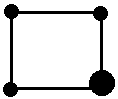
\includegraphics[width=0.15\linewidth]{image1.png}
\end{figure}
$$\text{Ш}(x,t)=\{(x,t),(x-h,t),(x,t+\tau),(x+h, t+\tau) \}.$$
С учетом этого шаблона можно построить разностную схему:
$$\begin{cases}
    y_t+a(\sigma\hat{y}_{\overline{x}}+(1-\sigma)y_{\overline{x}})=0,(x,t)\in \omega_{h \tau}\\
    y(x,0)=u_0(x),(x,t)\in \omega_{h \tau}\\
    y(0,t)=\mu(t),(x,t)\in \omega_{h \tau}
\end{cases}$$
или в индексной форме:
$$\begin{cases}
    \frac{y_k^{j+1}-y_k^j}{\tau}+a\Big(\sigma\frac{y_k^{j+1}-y_{k-1}^{j+1}}{h}+(1-\sigma)\frac{y_k^{j}-y_{k-1}^{j}}{h}\Big)=0,\\
    y_k^0=u_0(x),\\
    y_0^j=\mu^j.
\end{cases}$$
Для вычисления порядка данной разностной схемы необходимо найти порядок только уравнения, поскольку начальные и граничные условия аппроксимируются точно.
$$\psi_{h\tau}(x,t)=u_t+a(\sigma\hat{u}_{\overline{x}}+(1-\sigma)u_{\overline{x}})=\dot{u}+\frac{\tau}{2}\ddot{u}+a\Big[u'+\frac{h}{2}u''+\sigma \tau \dot{u}'+\sigma \tau \frac{h}{2}\dot{u}''\Big]+O(h^2) - \varphi=$$$$ = f+\frac{\tau}{2}\dot{f}+\frac{h}{2}f'-\varphi+a\tau\dot{u}'\Big(\sigma-\frac{1}{2}-\frac{h}{2\tau a}\Big)+O(h^2+\tau^2).$$
Таким образом, при $\varphi = f+\frac{\tau}{2}\dot{f}+\frac{h}{2}f',\ \sigma=\frac{1}{2}\Big(1+\frac{h}{a\tau}\Big)$ мы полчим РС порядка $O(h^2+\tau^2).$

\textbf{Спектральный метод.} Для того, чтобы исследовать разностную схему на устойчивость спектральным методом, необходимо в индексную форму построенной РС подставить выражение:
$$y_k^j=q^je^{ik\varphi}, \varphi \in [0,2\pi).$$
Подставим в уравнение разностной схемы:
$$\Big(q^{j+1}e^{ik\varphi}-q^je^{ik\varphi}\Big)+\frac{a\tau}{h}\Big(\sigma (q^{j+1}e^{ik\varphi}-q^{j+1}e^{i(k-1)\varphi})+(1-\sigma)(q^{j}e^{ik\varphi}-q^{j}e^{i(k-1)\varphi})\Big)=0.$$
Сократим на $q^{j+1}e^{i(k-1)\varphi}:$
$$(q-1)+\gamma\Big(\sigma(qe^{i\varphi}-q)+(1-\sigma)(e^{i\varphi}-1)\Big)=0.$$
Выразим отсюда $q$:
$$q=\frac{1-\gamma(1-\sigma)(e^{i\varphi}-1)}{1+\gamma\sigma(e^{i\varphi}-1)}.$$
Для спектрального метода необходимо выполнение условия: 
$$|q|^2\leq1,$$
следовательно, $$(1-\gamma(1-\sigma)(\cos(\varphi)-1))^2+(\gamma(1-\sigma)\sin(\varphi))^2\leq(1+\gamma\sigma(\cos(\varphi)-1))^2+(\gamma\sigma\sin(\varphi))^2,\Rightarrow$$$$\Rightarrow(1-\gamma(1-\sigma)(\cos(\varphi)-1)-1-\gamma\sigma(\cos(\varphi))-1)\cdot(1-\gamma(1-\sigma)(\cos(\varphi)-1)+1+\gamma\sigma(\cos(\varphi)-1))+$$$$+(\gamma(1-\sigma)\sin(\varphi)-\gamma\sigma\sin(\varphi))(\gamma(1-\sigma)\sin(\varphi)+\gamma\sigma\sin(\varphi))\leq0,\Rightarrow$$
$$\Rightarrow(-\gamma\cos(\varphi)+\gamma)(2-\gamma\cos(\varphi)+2\gamma\sigma\cos(\varphi)+\gamma-2\gamma\sigma)+(\gamma\sin(\varphi)-2\gamma\sigma\sin(\varphi))\gamma\sin(\varphi)\leq0\Rightarrow$$
$$\Rightarrow \gamma(1-\cos(\varphi))(2+\gamma(\cos(\varphi)-1)(2\sigma-1))+\gamma^2\sin^2(\varphi)(1-2\sigma)\leq0,\Rightarrow$$
$$\Rightarrow 2\gamma(1-\cos(\varphi))+\gamma^2(1-\cos(\varphi))^2(1-2\sigma)+\gamma^2\sin^2(\varphi)(1-2\sigma)\leq0, \Rightarrow$$
$$\Rightarrow 2\gamma(1-\cos(\varphi))+\gamma^2(1-2\cos(\varphi)\sin(\varphi)+\cos^2(\varphi))(1-2\sigma)+\gamma^2\sin^2(\varphi)(1-2\sigma)\leq0, \Rightarrow$$
$$\Rightarrow 2\gamma(1-\cos(\varphi))+\gamma^2(2-\sin(2\varphi))\cdot(1-2\sigma)\leq0,\Rightarrow$$
$$\Rightarrow 2\gamma(\gamma(1-2\sigma\cos(\varphi))+1)\leq0.$$
Рассмотрим два случая:

a) $a>0:$

Тогда $$1-2\sigma\cos(\varphi)\leq-\frac{1}{\gamma}, \Rightarrow \frac{1+\frac{1}{\gamma}}{2\cos(\varphi)}\leq\sigma, \Rightarrow\frac{\gamma+1}{2\gamma\cos(\varphi)}\leq\sigma, \Rightarrow \sigma\geq\frac{\gamma+1}{2\gamma}=\frac{1}{2}+\frac{h}{2a\tau}.$$
Таким образом, получили условие устойчивости при $a>0$.

б) $a<0:$

Тогда $$1-2\sigma\cos(\varphi)\geq-\frac{1}{\gamma},\Rightarrow\sigma\leq\frac{\gamma+1}{2\gamma\cos(\varphi)},\Rightarrow \sigma \leq\frac{\gamma+1}{2\gamma}=\frac{1}{2}+\frac{h}{2a\tau}.$$
Таким образом, получили условие устойчивости при $a<0$, однако это условие нас интересовать не будет, так как нам задано $a=10>0.$
\newpage

\subsection*{Задача 2}
\textbf{Постановка задачи}. Исследовать устойчивость РС с помощью принципа максимума.

\textbf{Решение задачи.} 
Для применения принципа максимум выпишем разностную схему, полученную в задании 1:
$$\begin{cases}
    y_t+a(\sigma\hat{y}_{\overline{x}}+(1-\sigma)y_{\overline{x}})=0,(x,t)\in \omega_{h \tau}\\
    y(x,0)=u_0(x),(x,t)\in \omega_{h \tau}\\
    y(0,t)=\mu(t),(x,t)\in \omega_{h \tau}
\end{cases}$$
или в индексной форме:
$$\begin{cases}
    \frac{y_k^{j+1}-y_k^j}{\tau}+a\Big(\sigma\frac{y_k^{j+1}+y_{k-1}^{j+1}}{h}-(1-\sigma)\frac{y_k^{j}-y_{k-1}^{j}}{h}\Big)=0,\\
    y_k^0=u_0(x),\\
    y_0^j=\mu^j.
\end{cases}$$
В качестве точки, отсносительно которой будем исследовать устойчивость, выберем точку $x=(x_k,t_{j+1}).$ Выразим из уравнения $y_k^j:$
$$y_k^{j+1}\Big(\frac{1}{\tau}+\frac{a\sigma}{h}\Big)=y_k^j\Big(\frac{1}{\tau}+\frac{(1-\sigma)a}{h}\Big)+y_{k-1}^j\frac{(1-\sigma)a}{h}+y_{k-1}^{j+1}\frac{a\sigma}{h}+\varphi_k^j.$$
Проверим выполнение условий устойчивости:
$$A(x)=\frac{1}{\tau}+\frac{a\sigma}{h}>0;\ B_1(x)=\frac{1}{\tau}+\frac{(1-\sigma)a}{h}>0;\ B_2(x)=\frac{(1-\sigma)a}{h}>0;\ B_3(x)=\frac{a\sigma}{h}>0;$$
Сократим на $A(x):$
$$A=1>0;\ B_1(x)=1-\frac{\sigma a\tau}{h+a\tau}>0\Rightarrow h>a\tau(\sigma-1);\ B_2(x)=\frac{(1-\sigma)a\tau}{h+a\sigma\tau}>0 \Rightarrow \sigma < 1;\ B_3(x)=\frac{a\sigma\tau}{h+a\sigma\tau}>0.$$
Таким образом, для устойчивости необходимо выполнение условий:
$$h>a\tau(\sigma-1);\ 0<\sigma<1;\ a>0.$$

\newpage
\subsection*{Задача 3}
\textbf{Постановка задачи.}

Выполнить машинную реализацию РС и проверить найденное условие устойчивости.

\textbf{Решение задачи.} 

\textbf{Спектральный метод.}
    Зададим нашу сетку узлов.

    \begin{tcolorbox}[breakable, size=fbox, boxrule=1pt, pad at break*=1mm,colback=cellbackground, colframe=cellborder]
\prompt{In}{incolor}{41}{\boxspacing}
\begin{Verbatim}[commandchars=\\\{\}]
\PY{k}{def} \PY{n+nf}{generate\PYZus{}grids}\PY{p}{(}\PY{n}{left\PYZus{}border}\PY{p}{,} \PY{n}{right\PYZus{}border}\PY{p}{,} \PY{n}{num\PYZus{}x\PYZus{}points}\PY{p}{,} \PY{n}{upper\PYZus{}bound}\PY{p}{,} \PY{n}{num\PYZus{}t\PYZus{}points}\PY{p}{)}\PY{p}{:}
    \PY{n}{h} \PY{o}{=} \PY{p}{(}\PY{n}{right\PYZus{}border}\PY{o}{\PYZhy{}}\PY{n}{left\PYZus{}border}\PY{p}{)} \PY{o}{/} \PY{n}{num\PYZus{}x\PYZus{}points}
    \PY{n}{nodes\PYZus{}x} \PY{o}{=} \PY{n}{np}\PY{o}{.}\PY{n}{linspace}\PY{p}{(}\PY{n}{left\PYZus{}border}\PY{p}{,} \PY{n}{right\PYZus{}border}\PY{p}{,} \PY{n}{num\PYZus{}x\PYZus{}points}\PY{o}{+}\PY{l+m+mi}{1}\PY{p}{)}
    \PY{n}{tau} \PY{o}{=} \PY{n}{upper\PYZus{}bound} \PY{o}{/} \PY{n}{num\PYZus{}t\PYZus{}points}
    \PY{n}{nodes\PYZus{}t} \PY{o}{=} \PY{n}{np}\PY{o}{.}\PY{n}{linspace}\PY{p}{(}\PY{l+m+mi}{0}\PY{p}{,} \PY{n}{upper\PYZus{}bound}\PY{p}{,} \PY{n}{num\PYZus{}t\PYZus{}points} \PY{o}{+} \PY{l+m+mi}{1}\PY{p}{)}
    
    \PY{k}{return} \PY{n}{nodes\PYZus{}x}\PY{p}{,} \PY{n}{nodes\PYZus{}t}\PY{p}{,} \PY{n}{h}\PY{p}{,} \PY{n}{tau}
\end{Verbatim}
\end{tcolorbox}

    Определим функцию \[u(x,t)=u_0(x-at)\] соответствующую точному решению
поставленной задачи Коши. Зададим \(a=10\) и \(u_0(x) = x^2\), а также
\(\mu(t)=100t^2\).

    \begin{tcolorbox}[breakable, size=fbox, boxrule=1pt, pad at break*=1mm,colback=cellbackground, colframe=cellborder]
\prompt{In}{incolor}{42}{\boxspacing}
\begin{Verbatim}[commandchars=\\\{\}]
\PY{k}{def} \PY{n+nf}{u}\PY{p}{(}\PY{n}{x}\PY{p}{,} \PY{n}{t}\PY{p}{,} \PY{n}{a}\PY{p}{,} \PY{n}{u\PYZus{}0}\PY{p}{)}\PY{p}{:}
    \PY{k}{return} \PY{n}{u\PYZus{}0}\PY{p}{(}\PY{n}{x} \PY{o}{\PYZhy{}} \PY{n}{a} \PY{o}{*} \PY{n}{t}\PY{p}{)}
    
\PY{n}{a} \PY{o}{=} \PY{l+m+mi}{10}

\PY{k}{def} \PY{n+nf}{u\PYZus{}0}\PY{p}{(}\PY{n}{x}\PY{p}{)}\PY{p}{:}
    \PY{k}{return} \PY{n}{x}\PY{o}{*}\PY{o}{*}\PY{l+m+mi}{2}

\PY{k}{def} \PY{n+nf}{mu}\PY{p}{(}\PY{n}{t}\PY{p}{)}\PY{p}{:}
    \PY{k}{return} \PY{l+m+mi}{100}\PY{o}{*}\PY{n}{t}\PY{o}{*}\PY{o}{*}\PY{l+m+mi}{2}
\end{Verbatim}
\end{tcolorbox}

    Определим построенную разностную схему: \[\begin{cases}
    \frac{y_k^{j+1}-y_k^j}{\tau}+a\Big(\sigma\frac{y_k^{j+1}-y_{k-1}^{j+1}}{h}+(1-\sigma)\frac{y_k^{j}-y_{k-1}^{j}}{h}\Big)=0,\\
    y_k^0=u_0(x),\\
    y_0^j=\mu^j.
\end{cases}\] Отсюда определим рекуррентную формулу:
\[y_k^{j+1}=(1+\sigma\gamma)^{(-1)}(y_k^j(1-(1-\sigma)\gamma)+y_{k-1}^j((1-\sigma)\gamma)+y_{k-1}^{j+1}\sigma\gamma),\ \gamma=\frac{a\tau}{h}\]
Пусть \(x\in [0,3],\ t\in[0,\frac{1}{4}]\), разобьем каждый из отрезков
на 5 частей. Также необходимо помнить, что для усточивости по принципу
максимума необходимо, чтобы \(\sigma\in (0,1)\), возьмем, например
\(\sigma=\frac{1}{2}\).

    \begin{tcolorbox}[breakable, size=fbox, boxrule=1pt, pad at break*=1mm,colback=cellbackground, colframe=cellborder]
\prompt{In}{incolor}{43}{\boxspacing}
\begin{Verbatim}[commandchars=\\\{\}]
\PY{k}{def} \PY{n+nf}{diff\PYZus{}scheme\PYZus{}solve}\PY{p}{(}\PY{n}{nodes\PYZus{}x}\PY{p}{,} \PY{n}{nodes\PYZus{}t}\PY{p}{,} \PY{n}{h}\PY{p}{,} \PY{n}{tau}\PY{p}{,} \PY{n}{sigma}\PY{p}{,} \PY{n}{u\PYZus{}0}\PY{p}{,} \PY{n}{a}\PY{p}{)}\PY{p}{:}
    \PY{n}{gamma} \PY{o}{=} \PY{n}{a} \PY{o}{*} \PY{n}{tau} \PY{o}{/} \PY{n}{h}
    \PY{n}{y} \PY{o}{=} \PY{n}{np}\PY{o}{.}\PY{n}{zeros}\PY{p}{(}\PY{p}{(}\PY{n+nb}{len}\PY{p}{(}\PY{n}{nodes\PYZus{}x}\PY{p}{)}\PY{p}{,} \PY{n+nb}{len}\PY{p}{(}\PY{n}{nodes\PYZus{}t}\PY{p}{)}\PY{p}{)}\PY{p}{)}

    \PY{k}{for} \PY{n}{k} \PY{o+ow}{in} \PY{n+nb}{range}\PY{p}{(}\PY{n+nb}{len}\PY{p}{(}\PY{n}{nodes\PYZus{}x}\PY{p}{)}\PY{p}{)}\PY{p}{:}
        \PY{n}{y}\PY{p}{[}\PY{n}{k}\PY{p}{,} \PY{l+m+mi}{0}\PY{p}{]} \PY{o}{=} \PY{n}{u\PYZus{}0}\PY{p}{(}\PY{n}{nodes\PYZus{}x}\PY{p}{[}\PY{n}{k}\PY{p}{]}\PY{p}{)}
        
    \PY{k}{for} \PY{n}{j} \PY{o+ow}{in} \PY{n+nb}{range}\PY{p}{(}\PY{n+nb}{len}\PY{p}{(}\PY{n}{nodes\PYZus{}t}\PY{p}{)}\PY{p}{)}\PY{p}{:}
        \PY{n}{y}\PY{p}{[}\PY{l+m+mi}{0}\PY{p}{,} \PY{n}{j}\PY{p}{]} \PY{o}{=} \PY{n}{mu}\PY{p}{(}\PY{n}{nodes\PYZus{}t}\PY{p}{[}\PY{n}{j}\PY{p}{]}\PY{p}{)}

    \PY{k}{for} \PY{n}{k} \PY{o+ow}{in} \PY{n+nb}{range}\PY{p}{(}\PY{n+nb}{len}\PY{p}{(}\PY{n}{nodes\PYZus{}x}\PY{p}{)}\PY{o}{\PYZhy{}}\PY{l+m+mi}{1}\PY{p}{)}\PY{p}{:}
        \PY{k}{for} \PY{n}{j} \PY{o+ow}{in} \PY{n+nb}{range}\PY{p}{(}\PY{n+nb}{len}\PY{p}{(}\PY{n}{nodes\PYZus{}t}\PY{p}{)}\PY{o}{\PYZhy{}}\PY{l+m+mi}{1}\PY{p}{)}\PY{p}{:}
            \PY{n}{y}\PY{p}{[}\PY{n}{k}\PY{p}{,} \PY{n}{j} \PY{o}{+} \PY{l+m+mi}{1}\PY{p}{]} \PY{o}{=} \PY{p}{(}\PY{l+m+mi}{1} \PY{o}{+} \PY{n}{sigma} \PY{o}{*} \PY{n}{gamma}\PY{p}{)}\PY{o}{*}\PY{o}{*}\PY{p}{(}\PY{o}{\PYZhy{}}\PY{l+m+mi}{1}\PY{p}{)} \PY{o}{*} \PY{p}{(}\PY{n}{y}\PY{p}{[}\PY{n}{k}\PY{p}{,} \PY{n}{j}\PY{p}{]} \PY{o}{*} \PY{p}{(}\PY{l+m+mi}{1} \PY{o}{\PYZhy{}} \PY{p}{(}\PY{l+m+mi}{1} \PY{o}{\PYZhy{}} \PY{n}{sigma}\PY{p}{)} \PY{o}{*} \PY{n}{gamma}\PY{p}{)} \PY{o}{+} \PY{n}{y}\PY{p}{[}\PY{n}{k}\PY{o}{\PYZhy{}}\PY{l+m+mi}{1}\PY{p}{,} \PY{n}{j}\PY{p}{]} \PY{o}{*} \PY{p}{(}\PY{p}{(}\PY{l+m+mi}{1} \PY{o}{\PYZhy{}} \PY{n}{sigma}\PY{p}{)} \PY{o}{*} \PY{n}{gamma}\PY{p}{)} \PY{o}{+} \PY{n}{y}\PY{p}{[}\PY{n}{k}\PY{o}{\PYZhy{}}\PY{l+m+mi}{1}\PY{p}{,} \PY{n}{j}\PY{o}{+}\PY{l+m+mi}{1}\PY{p}{]} \PY{o}{*} \PY{n}{sigma} \PY{o}{*} \PY{n}{gamma}\PY{p}{)}
            
    \PY{k}{return} \PY{n}{y}
\end{Verbatim}
\end{tcolorbox}

    С учетом предложенных отрезков, получаем следующие шаги \(h, \tau:\)

    \begin{tcolorbox}[breakable, size=fbox, boxrule=1pt, pad at break*=1mm,colback=cellbackground, colframe=cellborder]
\prompt{In}{incolor}{44}{\boxspacing}
\begin{Verbatim}[commandchars=\\\{\}]
\PY{n}{nodes\PYZus{}x}\PY{p}{,} \PY{n}{nodes\PYZus{}t}\PY{p}{,} \PY{n}{h}\PY{p}{,} \PY{n}{tau} \PY{o}{=} \PY{n}{generate\PYZus{}grids}\PY{p}{(}\PY{l+m+mi}{0}\PY{p}{,} \PY{l+m+mi}{3}\PY{p}{,} \PY{l+m+mi}{5}\PY{p}{,} \PY{l+m+mi}{1}\PY{o}{/}\PY{l+m+mi}{4}\PY{p}{,} \PY{l+m+mi}{5}\PY{p}{)}
\PY{n}{sigma} \PY{o}{=} \PY{l+m+mi}{1} \PY{o}{/} \PY{l+m+mi}{2}

\PY{n+nb}{print}\PY{p}{(}\PY{l+s+sa}{f}\PY{l+s+s1}{\PYZsq{}}\PY{l+s+s1}{h = }\PY{l+s+si}{\PYZob{}}\PY{n}{h}\PY{l+s+si}{\PYZcb{}}\PY{l+s+s1}{\PYZsq{}}\PY{p}{)}
\PY{n+nb}{print}\PY{p}{(}\PY{l+s+sa}{f}\PY{l+s+s1}{\PYZsq{}}\PY{l+s+s1}{tau = }\PY{l+s+si}{\PYZob{}}\PY{n}{tau}\PY{l+s+si}{\PYZcb{}}\PY{l+s+s1}{\PYZsq{}}\PY{p}{)}
\end{Verbatim}
\end{tcolorbox}

    \begin{Verbatim}[commandchars=\\\{\}]
h = 0.6
tau = 0.05
    \end{Verbatim}

    Проверим выполнение условий устойчивости при полученных
\(h=0.6,\  \tau=0.05,\ \sigma = \frac{1}{2}\), а именно
\[h>a\tau(\sigma-1).\]

    \begin{tcolorbox}[breakable, size=fbox, boxrule=1pt, pad at break*=1mm,colback=cellbackground, colframe=cellborder]
\prompt{In}{incolor}{45}{\boxspacing}
\begin{Verbatim}[commandchars=\\\{\}]
\PY{n+nb}{print}\PY{p}{(}\PY{n}{h} \PY{o}{\PYZgt{}} \PY{n}{a} \PY{o}{*} \PY{n}{tau} \PY{o}{*} \PY{p}{(}\PY{n}{sigma} \PY{o}{\PYZhy{}} \PY{l+m+mi}{1}\PY{p}{)}\PY{p}{)}
\end{Verbatim}
\end{tcolorbox}

    \begin{Verbatim}[commandchars=\\\{\}]
True
    \end{Verbatim}

    Условие выполняется, соответственно, по математическим обоснованиям
построенная РС должны быть устойчивой.

Построим график для решениея, полученного нашей разностной схемой и
точного решения.

    \begin{tcolorbox}[breakable, size=fbox, boxrule=1pt, pad at break*=1mm,colback=cellbackground, colframe=cellborder]
\prompt{In}{incolor}{46}{\boxspacing}
\begin{Verbatim}[commandchars=\\\{\}]
\PY{n}{y} \PY{o}{=} \PY{n}{diff\PYZus{}scheme\PYZus{}solve}\PY{p}{(}\PY{n}{nodes\PYZus{}x}\PY{p}{,} \PY{n}{nodes\PYZus{}t}\PY{p}{,} \PY{n}{h}\PY{p}{,} \PY{n}{tau}\PY{p}{,} \PY{n}{sigma}\PY{p}{,} \PY{n}{u\PYZus{}0}\PY{p}{,} \PY{n}{a}\PY{p}{)}

\PY{k}{for} \PY{n}{j}\PY{p}{,} \PY{n}{t} \PY{o+ow}{in} \PY{n+nb}{enumerate}\PY{p}{(}\PY{n}{nodes\PYZus{}t}\PY{p}{)}\PY{p}{:}
    \PY{n}{plt}\PY{o}{.}\PY{n}{figure}\PY{p}{(}\PY{n}{figsize}\PY{o}{=}\PY{p}{(}\PY{l+m+mi}{16}\PY{p}{,} \PY{l+m+mi}{8}\PY{p}{)}\PY{p}{)}
    \PY{n}{plt}\PY{o}{.}\PY{n}{plot}\PY{p}{(}\PY{n}{nodes\PYZus{}x}\PY{p}{[}\PY{p}{:}\PY{o}{\PYZhy{}}\PY{l+m+mi}{1}\PY{p}{]}\PY{p}{,} \PY{n}{y}\PY{p}{[}\PY{p}{:}\PY{o}{\PYZhy{}}\PY{l+m+mi}{1}\PY{p}{,} \PY{n}{j}\PY{p}{]}\PY{p}{,} \PY{n}{label}\PY{o}{=}\PY{l+s+s1}{\PYZsq{}}\PY{l+s+s1}{numerical solution}\PY{l+s+s1}{\PYZsq{}}\PY{p}{)}
    \PY{n}{plt}\PY{o}{.}\PY{n}{plot}\PY{p}{(}\PY{n}{nodes\PYZus{}x}\PY{p}{,} \PY{n}{u}\PY{p}{(}\PY{n}{nodes\PYZus{}x}\PY{p}{,} \PY{n}{t}\PY{p}{,} \PY{n}{a}\PY{p}{,} \PY{n}{u\PYZus{}0}\PY{p}{)}\PY{p}{,} \PY{n}{label}\PY{o}{=}\PY{l+s+s1}{\PYZsq{}}\PY{l+s+s1}{exact solution}\PY{l+s+s1}{\PYZsq{}}\PY{p}{)}
    \PY{n}{plt}\PY{o}{.}\PY{n}{grid}\PY{p}{(}\PY{k+kc}{True}\PY{p}{)}
    \PY{n}{plt}\PY{o}{.}\PY{n}{xlabel}\PY{p}{(}\PY{l+s+s1}{\PYZsq{}}\PY{l+s+s1}{x}\PY{l+s+s1}{\PYZsq{}}\PY{p}{)}
    \PY{n}{plt}\PY{o}{.}\PY{n}{ylabel}\PY{p}{(}\PY{l+s+s1}{\PYZsq{}}\PY{l+s+s1}{u(x,t)}\PY{l+s+s1}{\PYZsq{}}\PY{p}{)}
    \PY{n}{plt}\PY{o}{.}\PY{n}{title}\PY{p}{(}\PY{l+s+s1}{\PYZsq{}}\PY{l+s+s1}{Approximation in t\PYZus{}}\PY{l+s+s1}{\PYZsq{}} \PY{o}{+} \PY{n+nb}{str}\PY{p}{(}\PY{n}{j}\PY{p}{)} \PY{o}{+} \PY{l+s+s1}{\PYZsq{}}\PY{l+s+s1}{=}\PY{l+s+s1}{\PYZsq{}} \PY{o}{+} \PY{n+nb}{str}\PY{p}{(}\PY{n+nb}{round}\PY{p}{(}\PY{n}{t}\PY{p}{,} \PY{l+m+mi}{2}\PY{p}{)}\PY{p}{)}\PY{p}{)}
    \PY{n}{plt}\PY{o}{.}\PY{n}{legend}\PY{p}{(}\PY{p}{)}
    \PY{n}{plt}\PY{o}{.}\PY{n}{show}\PY{p}{(}\PY{p}{)}
\end{Verbatim}
\end{tcolorbox}

\begin{figure}
    \centering
    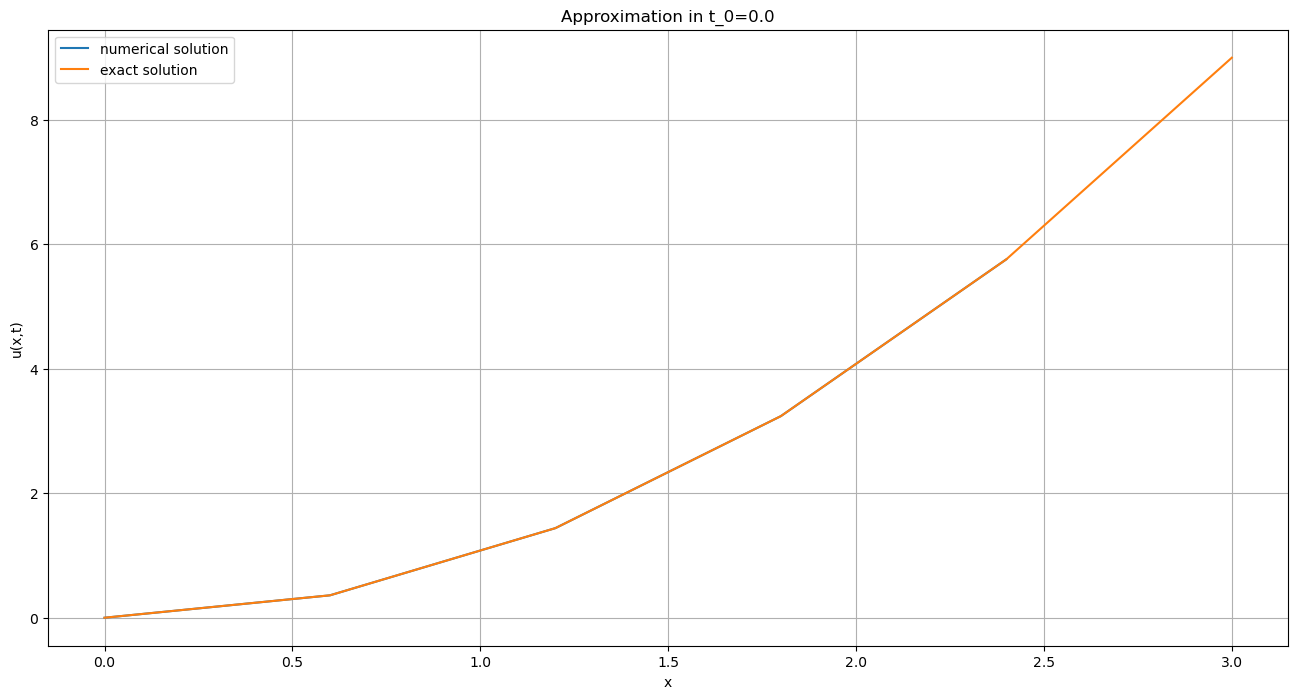
\includegraphics[width=0.15\linewidth]{output_13_0.png}
\end{figure}
    
    \begin{center}
    \adjustimage{max size={0.9\linewidth}{0.9\paperheight}}{output_13_1.png}
    \end{center}
    { \hspace*{\fill} \\}
    
    \begin{center}
    \adjustimage{max size={0.9\linewidth}{0.9\paperheight}}{output_13_2.png}
    \end{center}
    { \hspace*{\fill} \\}
    
    \begin{center}
    \adjustimage{max size={0.9\linewidth}{0.9\paperheight}}{output_13_3.png}
    \end{center}
    { \hspace*{\fill} \\}
    
    \begin{center}
    \adjustimage{max size={0.9\linewidth}{0.9\paperheight}}{output_13_4.png}
    \end{center}
    { \hspace*{\fill} \\}
    
    \begin{center}
    \adjustimage{max size={0.9\linewidth}{0.9\paperheight}}{output_13_5.png}
    \end{center}
    { \hspace*{\fill} \\}
    
    Как видим, с увеличением \(t\) точность решения ухужшается, но успешно
описывает точное решение, то есть можно сделать вывод, что схема
дейстивтельно оказалась устойчивой.


\textbf{Принцип максимума.}
Поскольку нам задано $a=10 > 0,$ то проверять устойчивость будем для случая $a >0,$ а именно неравенство:
\[\sigma\geq\frac{\gamma+1}{2\gamma}=\frac{1}{2}+\frac{h}{2a\tau}\]

    \begin{tcolorbox}[breakable, size=fbox, boxrule=1pt, pad at break*=1mm,colback=cellbackground, colframe=cellborder]
\prompt{In}{incolor}{47}{\boxspacing}
\begin{Verbatim}[commandchars=\\\{\}]
\PY{n+nb}{print}\PY{p}{(}\PY{n}{sigma} \PY{o}{\PYZgt{}} \PY{l+m+mi}{1}\PY{o}{/}\PY{l+m+mi}{2} \PY{o}{+} \PY{n}{h} \PY{o}{/} \PY{p}{(}\PY{l+m+mi}{2} \PY{o}{*} \PY{n}{a} \PY{o}{*} \PY{n}{tau}\PY{p}{)}\PY{p}{)}
\end{Verbatim}
\end{tcolorbox}

    \begin{Verbatim}[commandchars=\\\{\}]
False
    \end{Verbatim}

    Отсюда получаем, что для спектрального метода \(\sigma=\frac{1}{2}\) не
подходит, выберем \(\sigma = \frac{5}{4}\) и проверим условие.

    \begin{tcolorbox}[breakable, size=fbox, boxrule=1pt, pad at break*=1mm,colback=cellbackground, colframe=cellborder]
\prompt{In}{incolor}{48}{\boxspacing}
\begin{Verbatim}[commandchars=\\\{\}]
\PY{n}{sigma} \PY{o}{=} \PY{l+m+mi}{5} \PY{o}{/} \PY{l+m+mi}{4} 

\PY{n+nb}{print}\PY{p}{(}\PY{n}{sigma} \PY{o}{\PYZgt{}} \PY{l+m+mi}{1} \PY{o}{/} \PY{l+m+mi}{2} \PY{o}{+} \PY{n}{h} \PY{o}{/} \PY{p}{(}\PY{l+m+mi}{2} \PY{o}{*} \PY{n}{a} \PY{o}{*} \PY{n}{tau}\PY{p}{)}\PY{p}{)}
\end{Verbatim}
\end{tcolorbox}

    \begin{Verbatim}[commandchars=\\\{\}]
True
    \end{Verbatim}

    Проверим РС с новым параметром \(\sigma = \frac{5}{4}\).

    \begin{tcolorbox}[breakable, size=fbox, boxrule=1pt, pad at break*=1mm,colback=cellbackground, colframe=cellborder]
\prompt{In}{incolor}{50}{\boxspacing}
\begin{Verbatim}[commandchars=\\\{\}]
\PY{n}{y} \PY{o}{=} \PY{n}{diff\PYZus{}scheme\PYZus{}solve}\PY{p}{(}\PY{n}{nodes\PYZus{}x}\PY{p}{,} \PY{n}{nodes\PYZus{}t}\PY{p}{,} \PY{n}{h}\PY{p}{,} \PY{n}{tau}\PY{p}{,} \PY{n}{sigma}\PY{p}{,} \PY{n}{u\PYZus{}0}\PY{p}{,} \PY{n}{a}\PY{p}{)}

\PY{k}{for} \PY{n}{j}\PY{p}{,} \PY{n}{t} \PY{o+ow}{in} \PY{n+nb}{enumerate}\PY{p}{(}\PY{n}{nodes\PYZus{}t}\PY{p}{)}\PY{p}{:}
    \PY{n}{plt}\PY{o}{.}\PY{n}{figure}\PY{p}{(}\PY{n}{figsize}\PY{o}{=}\PY{p}{(}\PY{l+m+mi}{16}\PY{p}{,} \PY{l+m+mi}{8}\PY{p}{)}\PY{p}{)}
    \PY{n}{plt}\PY{o}{.}\PY{n}{plot}\PY{p}{(}\PY{n}{nodes\PYZus{}x}\PY{p}{[}\PY{p}{:}\PY{o}{\PYZhy{}}\PY{l+m+mi}{1}\PY{p}{]}\PY{p}{,} \PY{n}{y}\PY{p}{[}\PY{p}{:}\PY{o}{\PYZhy{}}\PY{l+m+mi}{1}\PY{p}{,} \PY{n}{j}\PY{p}{]}\PY{p}{,} \PY{n}{label}\PY{o}{=}\PY{l+s+s1}{\PYZsq{}}\PY{l+s+s1}{numerical solution}\PY{l+s+s1}{\PYZsq{}}\PY{p}{)}
    \PY{n}{plt}\PY{o}{.}\PY{n}{plot}\PY{p}{(}\PY{n}{nodes\PYZus{}x}\PY{p}{,} \PY{n}{u}\PY{p}{(}\PY{n}{nodes\PYZus{}x}\PY{p}{,} \PY{n}{t}\PY{p}{,} \PY{n}{a}\PY{p}{,} \PY{n}{u\PYZus{}0}\PY{p}{)}\PY{p}{,} \PY{n}{label}\PY{o}{=}\PY{l+s+s1}{\PYZsq{}}\PY{l+s+s1}{exact solution}\PY{l+s+s1}{\PYZsq{}}\PY{p}{)}
    \PY{n}{plt}\PY{o}{.}\PY{n}{grid}\PY{p}{(}\PY{k+kc}{True}\PY{p}{)}
    \PY{n}{plt}\PY{o}{.}\PY{n}{xlabel}\PY{p}{(}\PY{l+s+s1}{\PYZsq{}}\PY{l+s+s1}{x}\PY{l+s+s1}{\PYZsq{}}\PY{p}{)}
    \PY{n}{plt}\PY{o}{.}\PY{n}{ylabel}\PY{p}{(}\PY{l+s+s1}{\PYZsq{}}\PY{l+s+s1}{u(x,t)}\PY{l+s+s1}{\PYZsq{}}\PY{p}{)}
    \PY{n}{plt}\PY{o}{.}\PY{n}{title}\PY{p}{(}\PY{l+s+s1}{\PYZsq{}}\PY{l+s+s1}{Approximation in t\PYZus{}}\PY{l+s+s1}{\PYZsq{}} \PY{o}{+} \PY{n+nb}{str}\PY{p}{(}\PY{n}{j}\PY{p}{)} \PY{o}{+} \PY{l+s+s1}{\PYZsq{}}\PY{l+s+s1}{=}\PY{l+s+s1}{\PYZsq{}} \PY{o}{+} \PY{n+nb}{str}\PY{p}{(}\PY{n+nb}{round}\PY{p}{(}\PY{n}{t}\PY{p}{,} \PY{l+m+mi}{2}\PY{p}{)}\PY{p}{)}\PY{p}{)}
    \PY{n}{plt}\PY{o}{.}\PY{n}{legend}\PY{p}{(}\PY{p}{)}
    \PY{n}{plt}\PY{o}{.}\PY{n}{show}\PY{p}{(}\PY{p}{)}
\end{Verbatim}
\end{tcolorbox}

    \begin{center}
    \adjustimage{max size={0.9\linewidth}{0.9\paperheight}}{output_21_0.png}
    \end{center}
    { \hspace*{\fill} \\}
    
    \begin{center}
    \adjustimage{max size={0.9\linewidth}{0.9\paperheight}}{output_21_1.png}
    \end{center}
    { \hspace*{\fill} \\}
    
    \begin{center}
    \adjustimage{max size={0.9\linewidth}{0.9\paperheight}}{output_21_2.png}
    \end{center}
    { \hspace*{\fill} \\}
    
    \begin{center}
    \adjustimage{max size={0.9\linewidth}{0.9\paperheight}}{output_21_3.png}
    \end{center}
    { \hspace*{\fill} \\}
    
    \begin{center}
    \adjustimage{max size={0.9\linewidth}{0.9\paperheight}}{output_21_4.png}
    \end{center}
    { \hspace*{\fill} \\}
    
    \begin{center}
    \adjustimage{max size={0.9\linewidth}{0.9\paperheight}}{output_21_5.png}
    \end{center}
    { \hspace*{\fill} \\}
    
    На графиках видно, что  решение, полученное с помощью разностной схемы, описывает точное решение, что говорит об устойчивости нашей РС.

\end{document}